%Introduction to state charts
\section{Overview of State Machines} \label{sec:overviewstatechart}

Our proposed visual programming language involves using state machines with guarded edges. Our languages differs in a few concepts from the usual state machine syntax in order to support features of the hardware. To better understand these differences we will first introduce all the syntax and semantics of a \emphasize{Finite State Machines}\cite{booth} and \emphasize{UML2 State Machine Diagrams}\cite{UML2}.

A \emphasize{Finite State Machines}\cite{booth} defined as a diagram describing the behaviour of a discrete system.

\begin{definition}
A \emphasize{Finite State Machines} is defined as $M = \lbrace Q, I, Z, \delta, \omega, q_0\rbrace$

\label{def:statecharts}
\begin{itemize}
	\item $Q$: Set of states.
	\item $I$: Set of input symbols.
	\item $Z$: Set of output symbols.
	\item $\delta$: A state transition function: $I \times Q \rightarrow Q$. 
	\item $\omega$: An output function: $I \times Q \rightarrow Z$
	\item $q_0$: Starting state.
\end{itemize}
\end{definition}

A state represents a set of operating conditions. For example in figure \ref{fig:state_blink_light} the states are ``Light On'' and ``Light Off''.

\begin{figure}[htp]
    \centering
    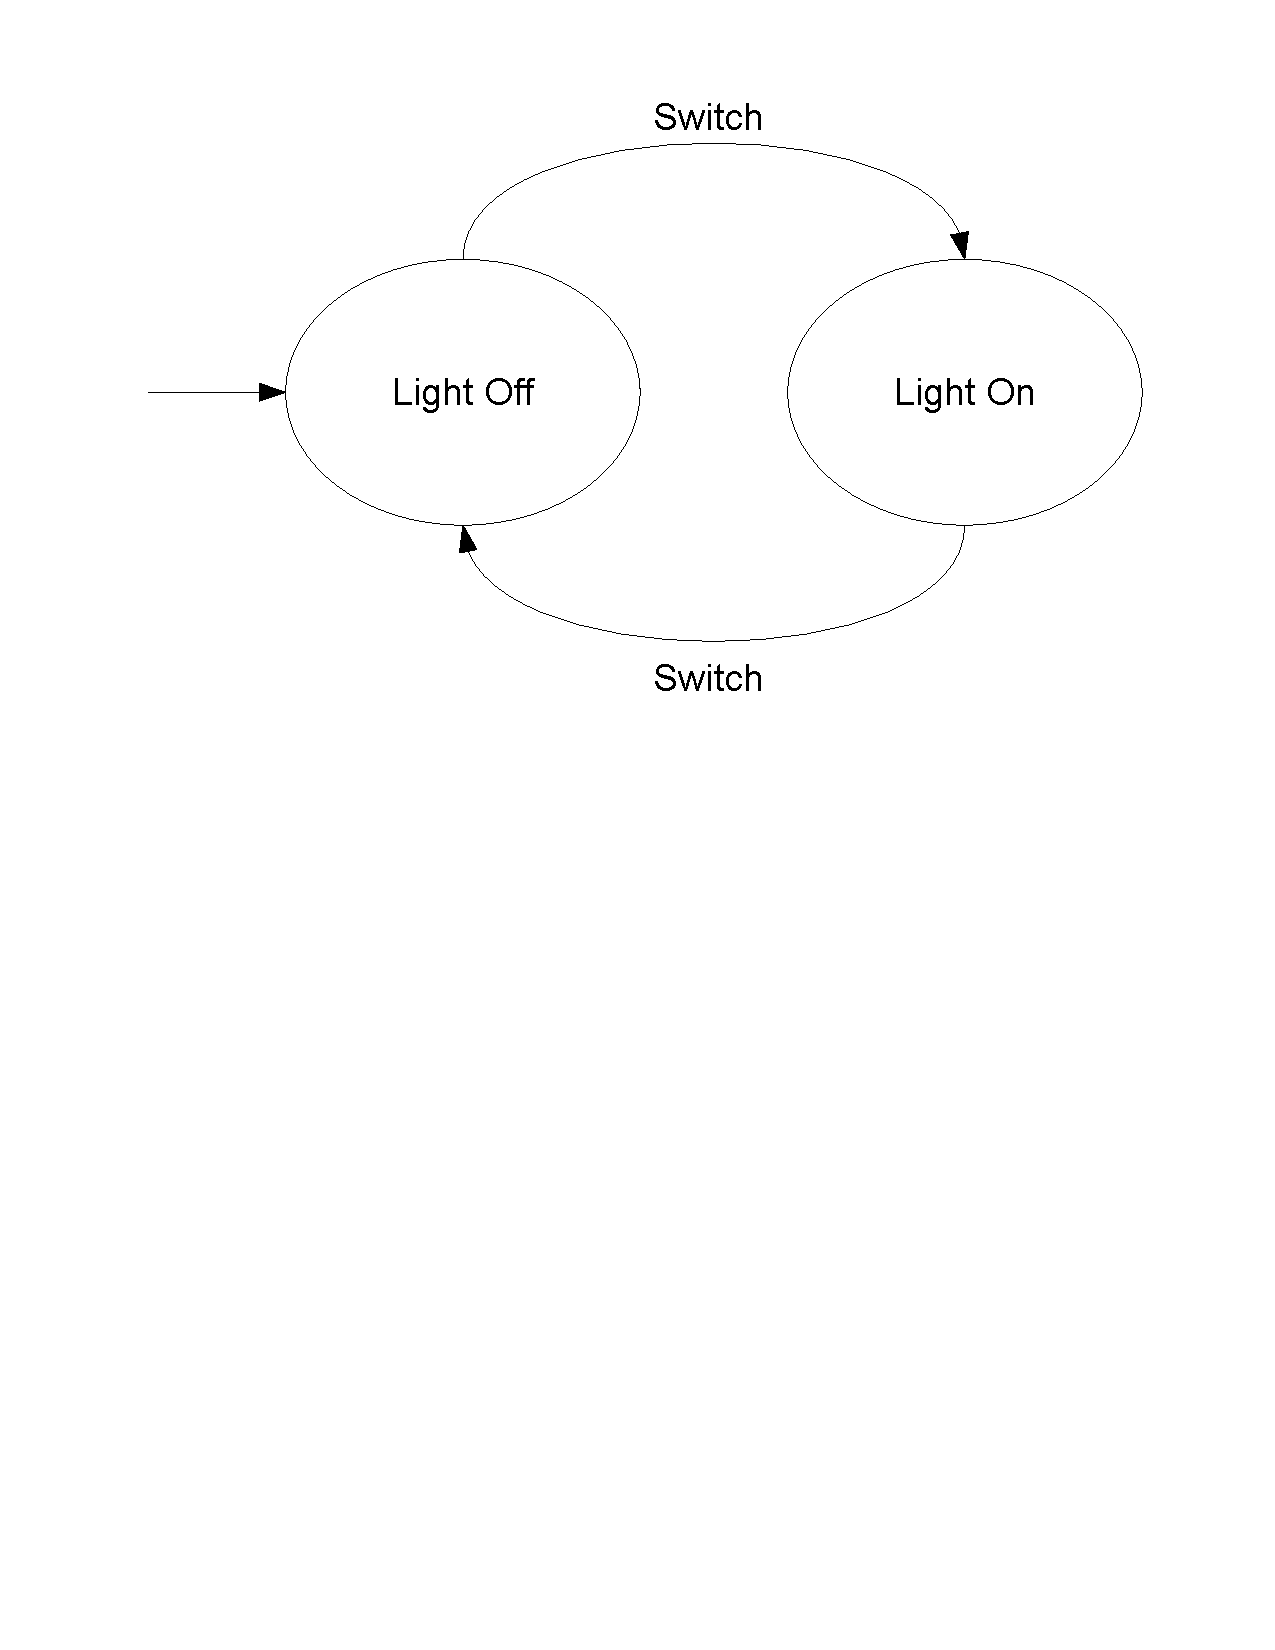
\includegraphics[trim= 10mm 150mm 10mm 10mm, clip, width=\imgmedium]{./images/state_blink_light.pdf}
    \caption{Simple Toggle Light}
    \label{fig:state_blink_light}
\end{figure}

Transitions are defined as functions $\delta(i,q_1) = q_2$ where inputs $i \in I$ a current state $q_1 \in Q$ and a next state $q_2 \in Q$.  Outputs can be formalized to $\omega(i,q_1)=z_1$ where $z_1 \in Z$. Machines that satisfy definition \ref{def:statecharts} are referred to as \emphasize{Mealy machines} \cite{booth}. A \emphasize{Moore machine} is the same as a defined above but output functions are only dependent on state. To obtain a \emphasize{Moore machine} from definition \ref{def:statecharts} we change our output function to $Q \rightarrow Z$. Although figure \ref{fig:state_moore_mealy} contains outputs for all edges, we can define ourselves a null output or a no change output in order to simulate an edge having no output as well. For purposes of the \plccharts language we do not require the power of a Mealy machine and thus we chose to stay with a simpler Moore machine. More details of this decision can be found in section \ref{sec:statechartsem}.

%diagram for Moore + Mealy state machines
\begin{figure}[htp]
    \centering
    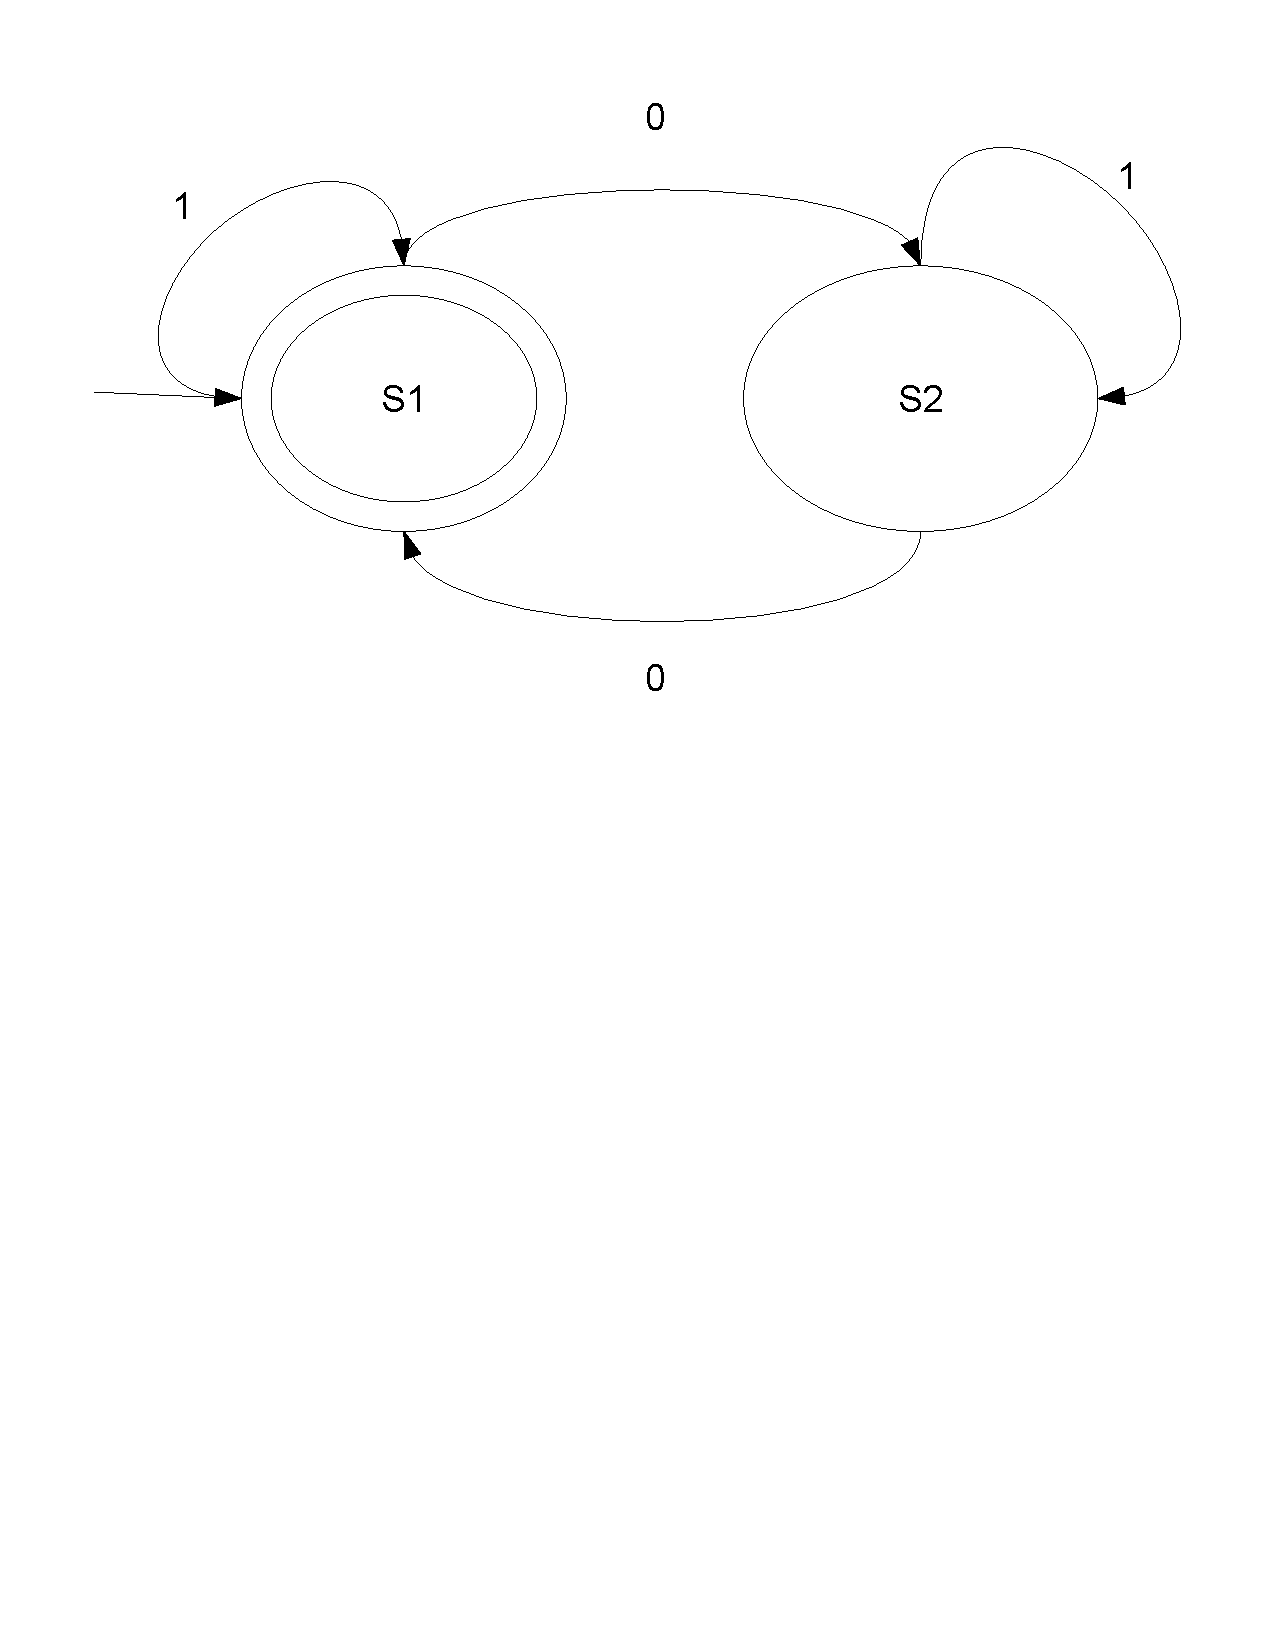
\includegraphics[trim= 15mm 150mm 15mm 10mm, clip, width=200pt]{./images/state_moore.pdf} 
    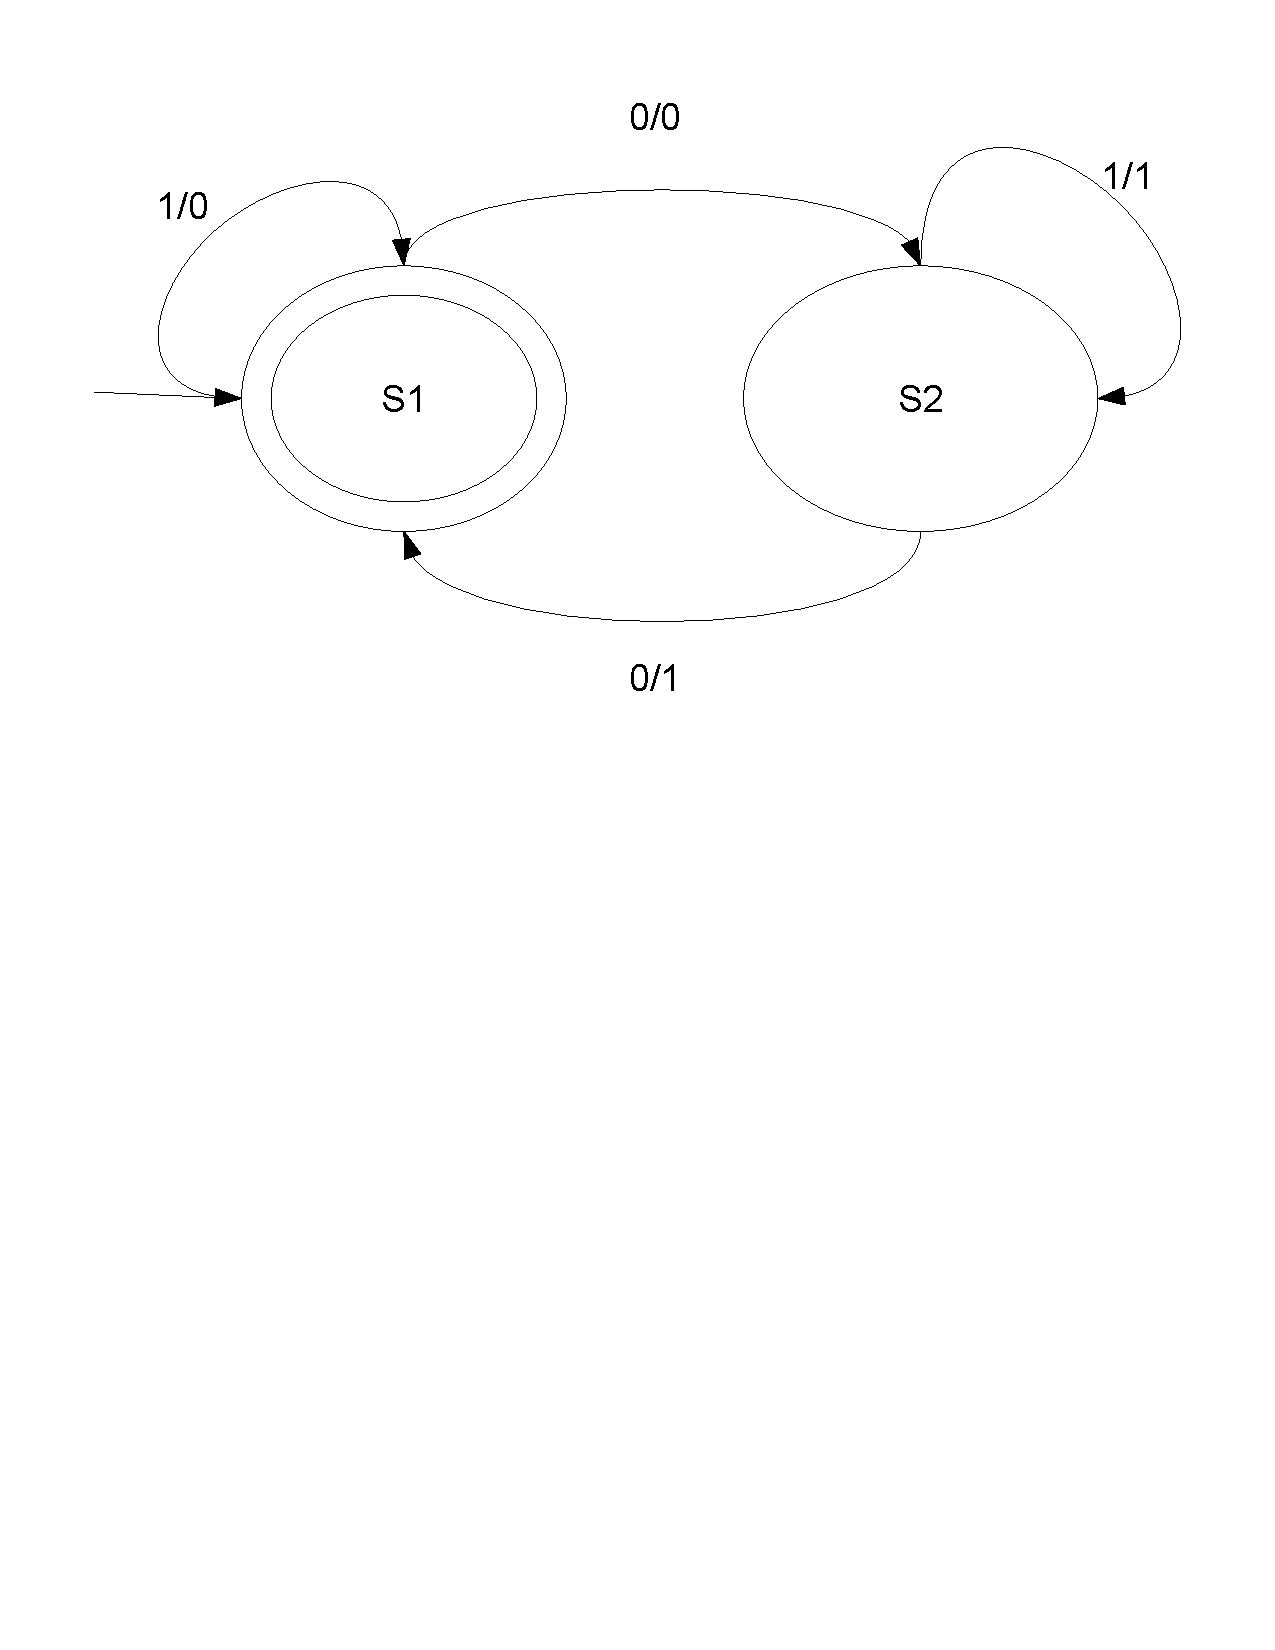
\includegraphics[trim= 15mm 150mm 15mm 10mm, clip, width=200pt]{./images/state_mealy.pdf}    
    \caption{Moore and Mealy State Machines}
    \label{fig:state_moore_mealy}
\end{figure}

There are several ways a starting state can be defined as seen in figure \ref{fig:state_moore_mealy}.
One such way is to draw a edge that has no state connected to its tail, this generally looks like an edge out of nowhere. In our system we choose to use the \emphasize{UML}\cite{UML2} symbol where the start state edge has a solid dot connected to the tail as shown in figure \ref{fig:state_uml_light}.

%diagram for UML state machines
\begin{figure}[htp]
    \centering
    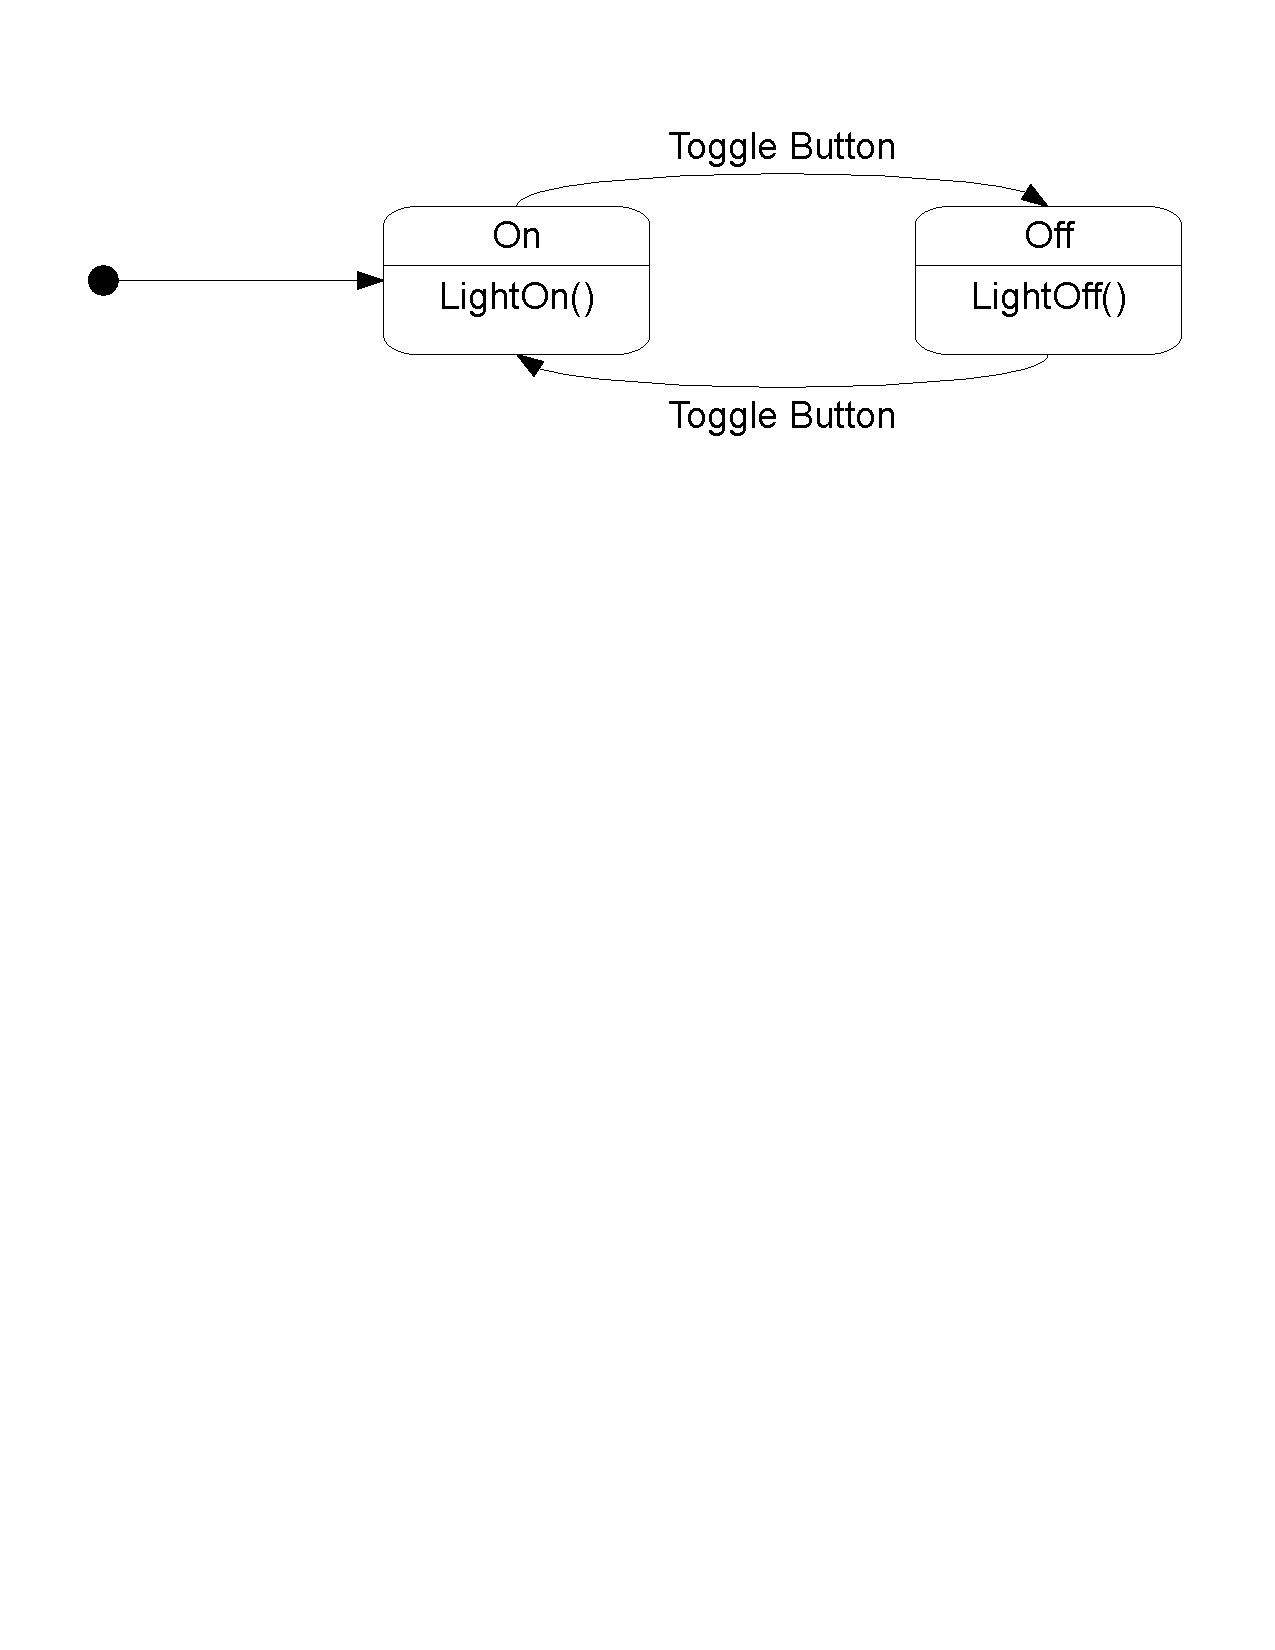
\includegraphics[trim= 15mm 200mm 15mm 10mm, clip, width=\imgmedium]{./images/state_uml_light.pdf} 
    \caption{UML State Diagram of a Toggle Light}
    \label{fig:state_uml_light}
\end{figure}

The \emphasize{UML State Diagrams}\cite{UML2} as shown in figure \ref{fig:state_uml_light} also allow for state titles in each state which can be seen at the top of each state. In addition, each state may contain executed actions that will occur. In this case ``LightOn()'' and ``LightOff()'' refer to executed routines that are called once the ``On'' and ``Off'' states are reached respectively. The behaviour is then once the state ``On'' is reached ``LightOn()'' is executed right away. More than one instruction to be executed can be listed and is understood that each instruction is executed sequentially\cite{UML2}.

%diagram for UML state machines
\begin{figure}[htp]
    \centering
    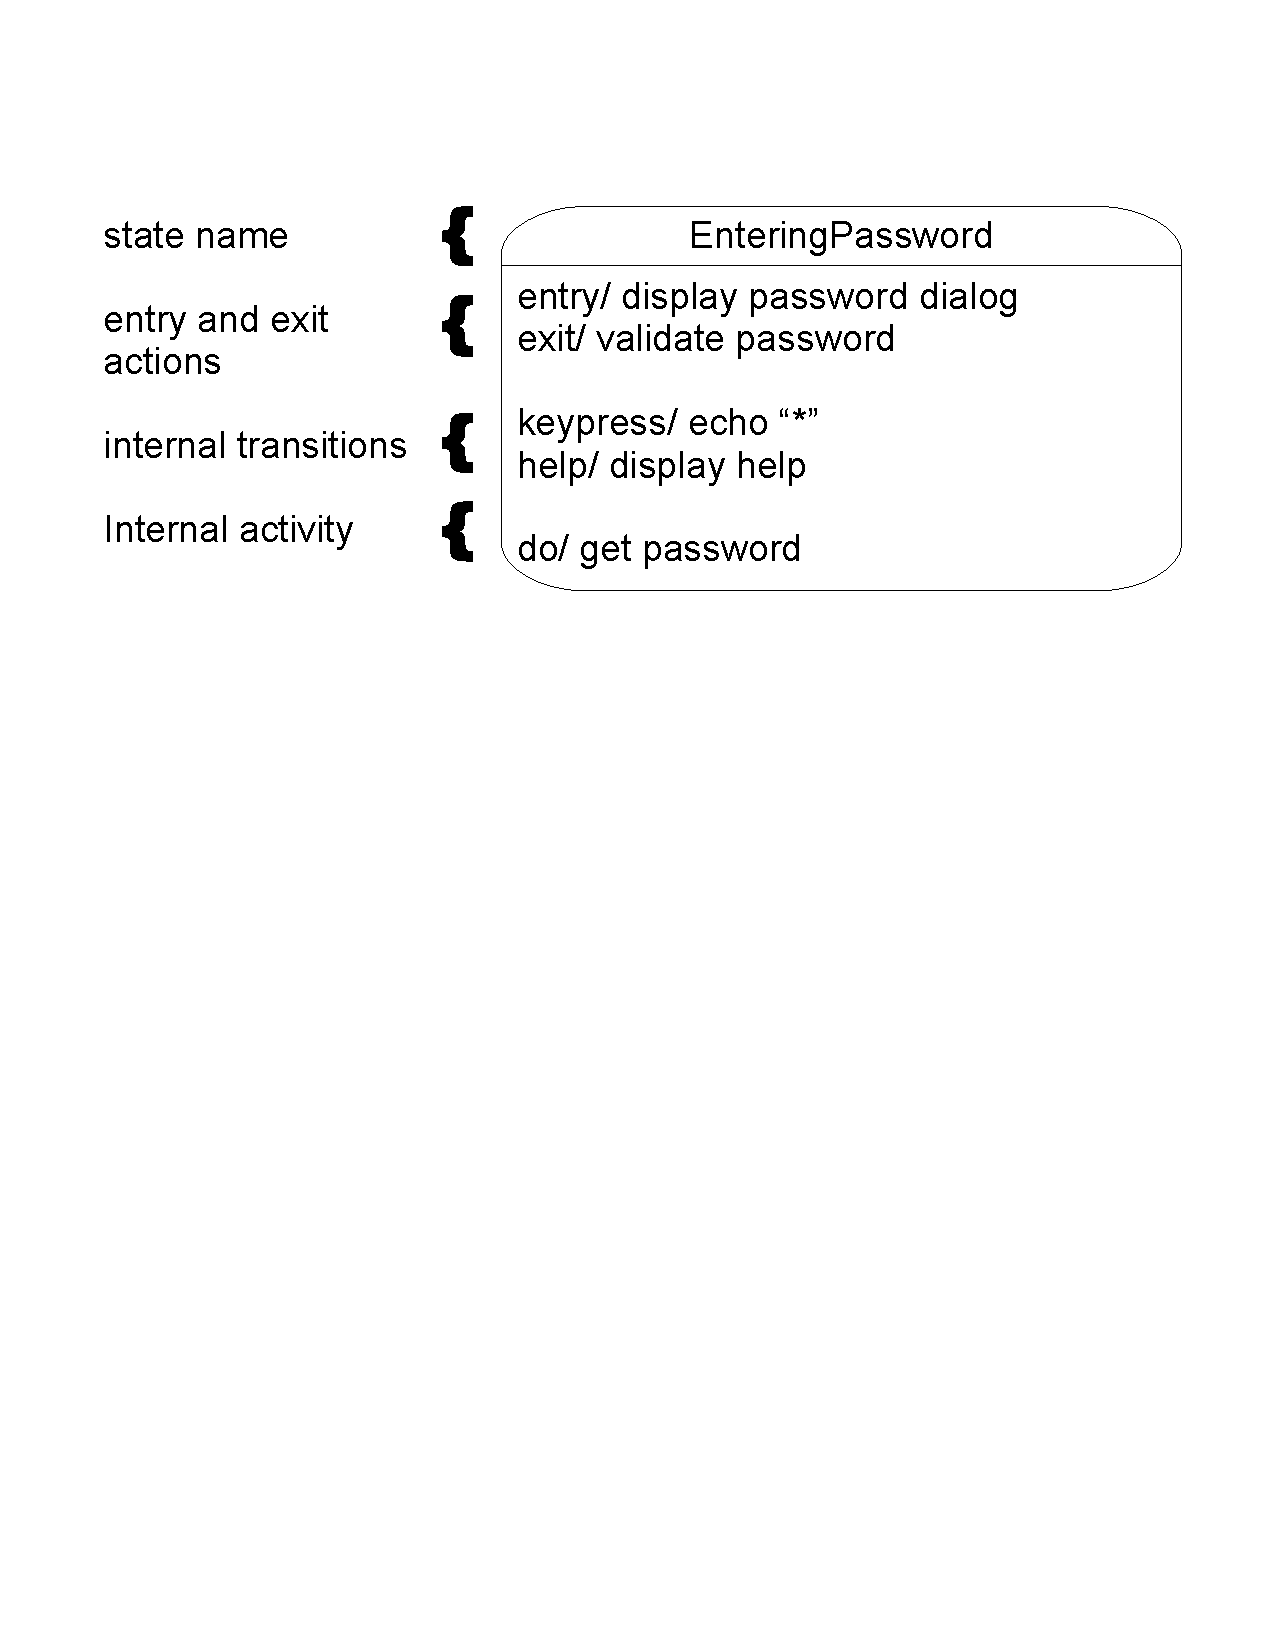
\includegraphics[trim= 15mm 175mm 15mm 10mm, clip, width=\imgmedium]{./images/state_uml2_syntax_21_4.pdf} 
    \caption{UML2 State Machine Diagram Syntax \cite{UML2}}
    \label{fig:state_uml2}
\end{figure}

The syntax shown in figure \ref{fig:state_uml_light} is \emphasize{UML2 State Machine Diagram}\cite{UML2}. \emphasize{UML2 State Machine Diagram}\cite{UML2} allows for additional information in each state. In figure \ref{fig:state_uml2} we note the additional features of  \emphasize{UML2 State Machine Diagram}\cite{UML2}. Each state in  \emphasize{UML2 State Machine Diagram}\cite{UML2} can contain the following information as defined in definition \ref{def:uml2}. This inherent flexibility makes UML2 more useful for representing more practical programs. In addition  \emphasize{UML2 State Machine Diagram}\cite{UML2} has a more precise syntax when compared to other methods of describing state machines namely when compared to \emphasize{Finite State Machines}\cite{booth}, and \emphasize{UML State Diagram}\cite{UML2}.

\begin{definition}
UML2 State Machine Diagram

\label{def:uml2}
\begin{itemize}
	\item \textbf{state name:} The state name is mandatory for each UML2 state in cases where this is the only information the horizontal divider may be omitted.
	\item \textbf{entry and exit actions:} Entry and exit options are optional, they are commonly used for initializers and finalizers that may occur upon each state.
	\item \textbf{internal transitions:} These optional fields refer to simple transitions that may happen in the state itself generally these are simple enough to not require a separate diagram.
	\item \textbf{internal activity:} Also optional but refer to activities that occur or are executed while in the state.
\end{itemize}
\end{definition}

